% Preamble
\documentclass{article}
\setlength\parindent{0pt}

% Packages
\usepackage{amsmath}
\usepackage{textcomp}
\usepackage{multirow}
\usepackage{algorithm}
\usepackage{algpseudocode}
\usepackage{tikz}
\usepackage[linktocpage]{hyperref}

\hypersetup{
    colorlinks   = true,
    urlcolor     = blue,
    linkcolor    = blue,
    citecolor   = red
}

\title{\textbf{ScreenView Protocol}}
\author{Josh Brown}

% Document
\begin{document}
    \maketitle

    \begin{abstract}
        ScreenView is a suite of cryptographical and application level networking protocols culminating to create a
        zero configuration end to end encrypted remote screen viewing and controlling software. ScreenView aims to
        replace TeamViewer, RDP, and VNC for many use cases while being more performant and more secure. ScreenView
        requires little set up and is just as easy or easier to set up than other solutions. ScreenView defines four different
        layers of protocols, each encapsulating all the layers below it. Cryptography for communication between peers
        and the server is based upon TLS 1.3 and Wireguard. End-to-end cryptography used for ALL communication between
        peers is based upon TLS-SRP. ScreenView end-to-end cryptography prevents man-in-the-middle attacks even if
        the intermediary server is compromised, unlike TeamViewer. Screen data is sent over UDP to achieve superior
        performance than TCP based solutions such as VNC. All UDP packets must be authenticated with keys established
        over TCP before a response is made by the server preventing amplification attacks. A congestion control
        mechanism is used to handle low bandwidth and poor networking conditions. Finally, ScreenView supports
        advanced use cases including file transfer, multiple displays, sharing specific windows, shared whiteboards,
        and clipboard transfer.
    \end{abstract}

    \newpage

    \tableofcontents
    \newpage


    \section{Definitions}

    The key words "MUST", "MUST NOT", "REQUIRED", "SHALL", "SHALL NOT",
    "SHOULD", "SHOULD NOT", "RECOMMENDED", "MAY", and "OPTIONAL" in this
    document are to be interpreted as described in \href{https://datatracker.ietf.org/doc/html/rfc2119}{RFC 2119}.

    \newpage

    \section{Introduction}

This section describes the high level overview of ScreenView. Terms used in this section are defined in other
sections.

\subsection{Application Layers}

The table belows is an abstract diagram of the different layers of ScreenView. Each layer encapsulates all the
below layers.

\begin{center}
    \begin{tabular}{|l|}
        \hline
        Transport Layer                                         \\
        | Server Encryption Layer                               \\
        || Server Communication Layer                           \\
        ||| E2EE (Peer $\leftrightarrow$ Peer) Encryption Layer \\
        |||| Host $\leftrightarrow$ Client Communication Layer  \\
        \hline
    \end{tabular}
\end{center}


The Transport Layer is the OSI Transport Layer level protocol for networking (TCP or UDP). The \hyperlink{section
.3}{Server
Encryption Layer} provides security between the Server and a Peer. \hyperlink{section.4}{The Server Communication
Layer} facilities communication between Peers and the Server. The \hyperlink{section.5}{E2EE (Peer
    $\leftrightarrow$ Peer) Encryption Layer} provides end-to-end encryption between a Peer and another Peer. The
\hyperlink{section.6}{Host $\leftrightarrow$ Client Communication Layer} facilities communication between a Peer and
another Peer.

    \section{Server Encryption Layer}

The Server Encryption Layer provides security for communication between Peers and the Server. TCP and UDP have
different security methods. UDP encryption depends on secrets established in the SVSC protocol and therefore can only
be begin after TCP encryption is already established.

\subsection{TCP}

The TCP Server Encryption Layer is heavily based on a simplification of TLS 1.3 as defined in
\href{https://datatracker.ietf.org/doc/html/rfc8446}{RFC8446}.

\subsubsection{PeerHello}

The Peer begins by sending a PeerHello message with their ephemeral public key.

\begin{center}
    Peer \textrightarrow\ Server\\
    \begin{tabular}{|c|c|c|}
        \hline
        \textbf{Bytes} & \textbf{Name} & \textbf{Value} \\
        \hline
        1              & type          & 1              \\
        \hline
        16             & public-key    &                \\
        \hline
    \end{tabular}
\end{center}

\begin{align*}
    &(E_{peer}^{pub},\,E_{peer}^{priv}) := \text{DH-Generate()}\\
    &\text{public-key} := E_{peer}^{pub}
\end{align*}

\subsubsection{ServerHello}

The Server replies with their certificate list. Like TLS, the is a certificate chain. This ensures that a MITM attack
between the Peer and the Server cannot occur. Additionally, the Server sends their ephemeral public key and a
signature. These ephemeral keys ensure perfect forward secrecy.

\begin{center}
    Server \textrightarrow\ Peer\\
    \begin{tabular}{|c|c|c|}
        \hline
        \textbf{Bytes}             & \textbf{Name}       & \textbf{Value} \\
        \hline
        1                          & type                & 2              \\
        \hline
        4                          & length              &                \\
        \hline
        3                          & certificates-length &                \\
        \hline
        \emph{certificates-length} & certificate\_list   &                \\
        \hline
        16                         & public-key          &                \\
        \hline
        variable                   & certificate-verify  &                \\
        \hline
    \end{tabular}
\end{center}

length is the size of the entire message not including the type. While not technically neccessary, it makes this
message easier to parse.\\

certificate\_list is defined in \href{https://datatracker.ietf.org/doc/html/rfc8446#section-4.4.2}{RFC8446
Section-4.4.2}.

\begin{align*}
    & (E_{serv}^{pub},\, E_{serv}^{priv}) := \text{DH-Generate()}\\
    & \text{public-key} := E_{serv}^{pub}
\end{align*}

certificate-verify is defined in \href{https://datatracker.ietf.org/doc/html/rfc8446#section-4.4
.3}{RFC8446 Section-4.4.3} with the following modification. The content that is signed is:\\

\begin{align*}
    \text{content} := \text{``SreenViewServerVerify''}\ ||\ 0\ ||\ E_{serv}^{pub}
\end{align*}

The Client MUST validate all signatures in accordance with the TLS spec.

\subsubsection{Transport Data Key Derivation}

The Server and Client derive their keys and initialize their nonces.

\begin{align*}
    & C_{peer} = \text{DH}(E_{serv}^{pub},\ E_{peer}^{priv})\\
    & C_{serv} = \text{DH}(E_{peer}^{pub},\ E_{serv}^{priv})\\
    & (T_{peer}^{send} = T_{serv}^{recv},\ T_{peer}^{recv} = T_{serv}^{send}) := \text{KDF}_2(C_{peer} = C_{serv},
    \ \epsilon) \\
    & N_{peer}^{send} = N_{serv}^{recv} = N_{peer}^{recv} = N_{serv}^{send} := 0
\end{align*}

\subsubsection{Subsequent Messages: Transport Data Messages}

All subsequent messages are encrypted and authenticated. On receiving a message, if authentication fails the message
MUST be dropped.

\begin{center}
    Peer $\leftrightarrow$ Server\\
    \begin{tabular}{|c|c|c|}
        \hline
        \textbf{Bytes}     & \textbf{Name} & \textbf{Value} \\
        \hline
        1                  & type          & 3              \\
        \hline
        2                  & data-length   &                \\
        \hline
        \emph{data-length} & data          &                \\
        \hline
    \end{tabular}
\end{center}

\begin{align*}
    & \text{data} := \text{AEAD}(T_{m}^{send}, N_{m}^{send}, P, \epsilon) \\
    & N_{m}^{send} := N_{m}^{send} + 1
\end{align*}

Where $P$ is the payload to be transported\\

$N_{m}$ is an 64 bit counter that MUST NOT wrap. After a transport message is sent, if $N_{m}$ equals
($2^{64}-1$) the TCP connection MUST be dropped. Subsequent TCP messages MUST NOT be sent. \\

\subsection{UDP}

UDP encryption and authentication rely on the \emph{session-id}, \emph{peer-id} and \emph{peer-key} values
established in a session
(described in \hyperlink{subsection.4.4}{4.4}). The Server (nor the Peer) MUST NOT
process or reply to any messages that don't pass authentication. This prevents an amplification attack.\\

\subsubsection{Transport Data Key Derivation}

The Server and Peer derive keys.

\begin{align*}
    &  G:= \text{session-id}                                                               \\
    &  H := \text{peer-id}                                                                \\
    &  J := \text{peer-key}                                                              \\
    &  (V_{peer}^{send} = V_{serv}^{recv}, V_{peer}^{recv} = V_{serv}^{send}) := \text{KDF}_2(\text{HASH}(G\,
    ||\, H\,||\, J), \epsilon)                                        \\
    &   M_{peer}^{send} = M_{serv}^{recv} = M_{peer}^{recv} = M_{serv}^{send} := 0
\end{align*}

\subsubsection{Transport Data Messages}

\begin{center}
    Peer \textrightarrow Server\\
    \begin{tabular}{|c|c|c|}
        \hline
        \textbf{Bytes}                & \textbf{Name}  & \textbf{Value} \\
        \hline
        1                             & type           & 4              \\
        \hline
        16                            & \emph{peer-id} &                \\
        \hline
        8                             & counter        &                \\
        \hline
        $\text{UDP length} - 8$ bytes & data           &                \\
        \hline
    \end{tabular}
\end{center}

\begin{center}
    Server \textrightarrow Peer\\
    \begin{tabular}{|c|c|c|}
        \hline
        \textbf{Bytes}                & \textbf{Name} & \textbf{Value} \\
        \hline
        1                             & type          & 5              \\
        \hline
        8                             & counter       &                \\
        \hline
        $\text{UDP length} - 8$ bytes & data          &                \\
        \hline
    \end{tabular}
\end{center}


\begin{align*}
    & \text{data} := \text{AEAD}(V_{m}^{send}, M_{m}^{send}, P, \epsilon)\\
    & \text{counter} := M_{m}^{send}\\
    & M_{m}^{send} := M_{m}^{send} + 1
\end{align*}


Where $P$ is the payload to be transported\\

$M_{m}$ is an 64 bit counter that MUST NOT wrap. After a transport message is sent, if $M_{m}$ equals
($2^{64}-1$) the TCP connection MUST be dropped. Subsequent UDP messages MUST NOT be sent. \\



    \section{ScreenView Server Communication (SVSC) Protocol }

The SVSC protocol is the Server Communication Layer protocol used for Peers to interact with the relay server,
Server. Peers can lease an ID as well as begin a session with another Peer. Once a session is established, Peers can
forward messages to another Peer. Unless otherwise noted, all messages MUST occur over TCP.\\

With the exception of the \hyperlink{subsection.4.2}{Handshake} messages. All SVSC messages' first byte contain a
number to indicate
the message type.

\subsection{Definitions}

\begin{itemize}
    \item Peer - denotes a client in classical server/client environment
    \item Server - The intermediary server used for routing and proxying data between
\end{itemize}

\subsection{Handshake}

\subsubsection{ProtocolVersion}

Handshaking begins with the Server sending the Peer a ProtocolVersion message. This lets the server know
the version supported by the Host. the ProtocolVersion message consists of 12 bytes interpreted as a string of ASCII
characters in the format
"SVSC xxx.yyy" where xxx and yyy are the major and minor version numbers, padded with zeros.

\begin{center}
    Server \textrightarrow\ Peer\\
    \begin{tabular}{|c|c|c|}
        \hline
        \textbf{Bytes} & \textbf{Name} & \textbf{Value}            \\
        \hline
        11             & version       & ``\texttt{SVSC 001.000}'' \\
        \hline
    \end{tabular}
\end{center}

The Peer replies back either \texttt{0} to indicate the version is not acceptable and that the handshake has
failed or \texttt{1} if the version is acceptable to the Peer and the handshake as succeeded. If \texttt{0} is sent, all
communication MUST cease and the TCP connection MUST be terminated.

\begin{center}
    Peer \textrightarrow\ Server\\
    \begin{tabular}{|c|c|c|}
        \hline
        \textbf{Bytes} & \textbf{Name} & \textbf{Value} \\
        \hline
        1              & ok            & 0 or 1         \\
        \hline
    \end{tabular}
\end{center}

\subsection{Leasing}

A lease is a temporary assignment of an ID to a Peer. The ID format and generation is discussed in
\hyperlink{subsubsection.4.3.5}{4.3.5}. A maximum of 1 ID can be leased per TCP connection. ID generation MUST be
rate limited to prevent ID exhaustion. Rate limiting rules are out of scope for this protocol, however some
suggestions are listed in \hyperlink{subsubsection.4.3.6}{4.3.6}.

\subsubsection{LeaseRequest}

A \emph{LeaseRequest} message requests a lease of an ID.

\begin{center}
    Peer \textrightarrow\ Server\\
    \begin{tabular}{|c|c|c|}
        \hline
        \textbf{Bytes} & \textbf{Name} & \textbf{Value} \\
        \hline
        1              & type          & 1              \\
        \hline
        1              & has-cookie    & 0 or 1         \\
        \hline
        \multicolumn{3}{|c|}{\textbf{Below only if \emph{has-cookie} is 1} } \\
        \hline
        24             & cookie        &                \\
        \hline
    \end{tabular}
\end{center}

If a Peer would like to request an ID it had previously been issued after expiration, it may include the cookie
value it received in the LeaseResponse. There is no guarantee that the Peer will receive the same ID or that the Server
will even consider the cookie value.

\subsubsection{LeaseResponse}

A LeaseResponse message is a response to a LeaseRequest. If has-cookie is 1, a Server MAY consider the cookie value
in LeaseRequest or completely
ignore it.

\begin{center}
    Server \textrightarrow\ Peer\\
    \begin{tabular}{|c|c|c|}
        \hline
        \textbf{Bytes} & \textbf{Name} & \textbf{Value} \\
        \hline
        1              & type          & 2              \\
        \hline
        1              & accepted      & 0 or 1         \\
        \hline
        \multicolumn{3}{|c|}{\textbf{Below only if \emph{accepted} is 1} } \\
        \hline
        4              & id            &                \\
        \hline
        24             & cookie        &                \\
        \hline
        8              & expiration    &                \\
        \hline
    \end{tabular}
\end{center}

\emph{expiration} is a 64 bit Unix timestamp representing the expiry of lease. Disconnection of a Peer (e.g,
the TCP connection is dropped) does not end a lease.\\

\emph{cookie} a 128 bit value. The generation of this value is discussed in \hyperlink{subsubsection.4.2.7}{4.2
.7}.\\

Consideration of the cookie value MUST have no effect on the the value of accepted. That is, if the
request is for a specific ID (implied by the presence of a cookie value and a has-cookie value equal to 1
in the LeaseRequest) and the ID requested is not available, the Server SHOULD respond with a different
available ID and an accepted value of 1 (assuming an ID is available). accepted MUST only be 0 if no IDs are left,
for rate limiting reasons, or some other reasons unrelated to the cookie value.

\subsubsection{LeaseExtensionRequest}

A LeaseExtensionRequest message is used to extend a lease. Before a lease has expired, the Peer can
request a lease extension. The Server can accept or deny this request. The Peer SHOULD send this message no earlier
than as soon as 50 percent of the lease duration has expired.

\begin{center}
    Peer \textrightarrow\ Server\\
    \begin{tabular}{|c|c|c|}
        \hline
        \textbf{Bytes} & \textbf{Name} & \textbf{Value} \\
        \hline
        1              & type          & 3              \\
        \hline
        24             & cookie        &                \\
        \hline
    \end{tabular}
\end{center}

\subsubsection{LeaseExtensionResponse}

A LeaseExtensionResponse message is a response to a LeaseExtensionRequest.

\begin{center}
    Server \textrightarrow\ Peer\\
    \begin{tabular}{|c|c|c|}
        \hline
        \textbf{Bytes} & \textbf{Name}  & \textbf{Value} \\
        \hline
        1              & type           & 4              \\
        \hline
        1              & extended       & 0 or 1         \\
        \hline
        \multicolumn{3}{|c|}{\textbf{Below only if \emph{extended} is 1} } \\
        \hline
        8              & new-expiration &                \\
        \hline
    \end{tabular}
\end{center}

\emph{new-expiration} is a 64 bit Unix timestamp representing the expiry of lease.

\subsubsection{ID Generation}

An ID is a 26 to 33 bit decimal number. This comes out to about up to 8 to 10 decimal digits, respectively. The
Server may scale the keyspace depending on current usage. For optimal user experience while maintaining
efficiency, the Server MUST only use keyspaces between 26 bits and 33 bits for ID generation. ID generation must
also be uniformly random. All active IDs must be stored on the server. New IDs MUST be unique. ID generation MAY
occur using the below
algorithm:\\

Let $S$ represents a set of all active IDs, $B$ be a number of bits between 26 and 33, and $generate(x)$ be a
functions that returns a $x$ uniformly random bits.

\begin{algorithm}
    \caption{ID generation}
    \begin{algorithmic}
        \State $id$
        \Repeat
            \State $id\gets generate(B)$
        \Until{$id\notin S$}
        \State $S\gets S\cup \{id\}$
        \State \textbf{return} $id$
    \end{algorithmic}
\end{algorithm}

\subsubsection{Rate Limits}

To prevent ID exhaustion, rate limits SHOULD be in place. TCP is used for LeaseRequests so IP addresses
can not be spoofed. However, using proxy services such as Tor, simple IP based rate limits are likely not
entirely sufficient. Servers MAY want to block all known proxy IP addresses.

\subsubsection{Cookie Value}

A \emph{cookie} value is a 128 bit value used for authentication in LeaseExtensionRequest and
LeaseRequest messages. Specific generation of a cookie is out of scope, however care must be taken
to ensure it is not predictable or exploitable. This value MAY be simply a random 24 byte key, HMAC-SHA1($id$,
$key$) $||$ $id$, or something else entirely.

\subsection{Sessions}

A session is a connection between two Peers. At least one Peer must have an ID. A Peer can have a maximum of one
session at any time. Immediately after receiving a EstablishSessionResponse message with a status
of 0 or a EstablishSessionNotification message a Peer MUST establish UDP connection by sending a
Keepalive message as defined in \hyperlink{subsection.4.5}{4.5}. Failure to do so MAY result in dropped
SessionData* packets.

\subsubsection{EstablishSessionRequest}

An EstablishSessionRequest message is a Peer request to establish a session with another Peer.

\begin{center}
    Peer \textrightarrow\ Server\\
    \begin{tabular}{|c|c|c|c|}
        \hline
        \textbf{Bytes} & \textbf{Name} & \textbf{Value} & \textbf{Description}                                 \\
        \hline
        1              & type          & 5              &                                                      \\
        \hline
        4              & lease-id      &                & The ID of the Peer to establish this connection with \\
        \hline
    \end{tabular}
\end{center}

\subsubsection{EstablishSessionResponse}

An EstablishSessionResponse message is a response to EstablishSessionRequest.

\begin{center}
    Server \textrightarrow\ Peer\\
    \begin{tabular}{|c|c|c|c|}
        \hline
        \textbf{Bytes} & \textbf{Name} & \textbf{Value} & \textbf{Description}                       \\
        \hline
        1              & type          & 6              &                                            \\
        \hline
        4              & lease-id      &                & the ID of the Peer attempted to connect to \\
        \hline
        1              & status        & 0-5            & described below                            \\
        \hline
        \multicolumn{4}{|c|}{\textbf{Below only if \emph{status} is 0} } \\
        \hline
        16             & session-id    &                & described below                            \\
        \hline
        16             & peer-id       &                & described below                            \\
        \hline
        16             & peer-key      &                & described below                            \\
        \hline
    \end{tabular}
\end{center}

\emph{status} can have the following values:

\begin{center}
    \begin{tabular}{|c|c|}
        \hline
        \textbf{Value} & \textbf{Description}                 \\
        \hline
        0              & session establishment was successful \\
        \hline
        1              & ID not found                         \\
        \hline
        2              & Peer is offline                      \\
        \hline
        3              & Peer is busy                         \\
        \hline
        4              & You are busy                         \\
        \hline
        5              & Other error                          \\
        \hline
    \end{tabular}
\end{center}

A Peer may be considered offline if, for example, an unexpired ID has been assigned to them and then the TCP
connection is dropped.\\

\emph{session-id} is a 128 bit random value used for session identification\\

\emph{peer-id} is a 128 bit random value used to authentication a Peer for a given session. A Peer's peer-key MUST
never be revealed to anyone but the Peer it belongs to (and the Server that generated it)
for security reasons.\\

\subsubsection{EstablishSessionNotification}

A EstablishSessionNotification notifies a Peer that a session has been established with them.

\begin{center}
    Server \textrightarrow\ Host\\
    \begin{tabular}{|c|c|c|c|}
        \hline
        \textbf{Bytes} & \textbf{Name} & \textbf{Value} & \textbf{Description}                                \\
        \hline
        1              & type          & 7              &                                                     \\
        \hline
        16             & session-id    &                & described in \hyperlink{subsubsection.4.4.2}{4.4.2} \\
        \hline
        16             & peer-id       &                & described in \hyperlink{subsubsection.4.4.2}{4.4.2} \\
        \hline
        16             & peer-key      &                & described in \hyperlink{subsubsection.4.4.2}{4.4.2} \\
        \hline
    \end{tabular}
\end{center}

peer-id and peer-key are the id and key of the Peer being notified NOT the id and key of the Peer they are connecting
to.

\subsubsection{SessionEnd}

A \emph{SessionEnd} message is used to terminate a session. Once a Server receives a SessionEnd message, the Server
MUST immediately stop forwarding messages and send a SessionEndNotification to the other Peer. The Peer must ignore
any SessionDataPacket message received after this.

\begin{center}
    Peer \textrightarrow\ Server\\
    \begin{tabular}{|c|c|c|c|}
        \hline
        \textbf{Bytes} & \textbf{Name} & \textbf{Value} & \textbf{Description} \\
        \hline
        1              & type          & 8              &                      \\
        \hline
    \end{tabular}
\end{center}

\subsubsection{SessionEndNotification}

A SessionEndNotification notifies a Peer that a session has ended. If a Peer sends a SessionEnd
message, the Server MUST send a SessionEndNotification message to a Peer. The Peer must ignore
any SessionDataPacket message received after this

\begin{center}
    Server \textrightarrow\ Peer\\
    \begin{tabular}{|c|c|c|c|}
        \hline
        \textbf{Bytes} & \textbf{Name} & \textbf{Value} & \textbf{Description} \\
        \hline
        1              & type          & 9              &                      \\
        \hline
    \end{tabular}
\end{center}

\subsubsection{SessionDataSend - TCP/UDP}

A SessionDataSend is a message from a Peer intended to be forwarded to the Peer on the other side of the
session. If a connection is not available (e.g. UDP was dropped or never established) for
SessionDataReceive message to be sent to the other Peer, the SessionDataSend message is silently dropped.

\begin{center}
    Peer \textrightarrow\ Server\\
    \begin{tabular}{|c|c|c|c|}
        \hline
        \textbf{Bytes} & \textbf{Name} & \textbf{Value} & \textbf{Description}           \\
        \hline
        1              & type          & 10             &                                \\
        \hline
        3              & data-length   &                & length of the content in bytes \\
        \hline
        data-length    & data          &                & data to be forwarded           \\
        \hline
    \end{tabular}
\end{center}

\subsubsection{SessionDataReceive - TCP/UDP}

A SessionDataReceive is a message being forwarded to a Peer from the Peer on the other side of the
session. The Server SHOULD forward the message along the same transport as it was received.

\begin{center}
    Server \textrightarrow\ Peer\\
    \begin{tabular}{|c|c|c|c|}
        \hline
        \textbf{Bytes} & \textbf{Name} & \textbf{Value} & \textbf{Description}           \\
        \hline
        1              & type          & 11             &                                \\
        \hline
        3              & data-length   &                & length of the content in bytes \\
        \hline
        data-length    & data          &                & data to be forwarded           \\
        \hline
    \end{tabular}
\end{center}

\subsection{Keepalive - TCP/UDP}

For each transport (TCP and UDP), if no message has been sent in \emph{KeepaliveTimeout} a Server sends a keepalive
message over the respective transport. The Peer MUST respond with another Keepalive message.\\

For TCP, if a \emph{KeepaliveTimeout} response is not received by the Server in
double \emph{KeepaliveTimeout} seconds the TCP connection is considered dropped.\\

For UDP, if a \emph{KeepaliveTimeout} response is not received by the Server in
half  \emph{KeepaliveTimeout} seconds another \emph{Keepalive} message is sent. If a response is not received in
an additional half \emph{KeepaliveTimeout} seconds, the UDP connection is considered dropped.

\begin{center}
    Server $\leftrightarrow$ Peer\\
    \begin{tabular}{|c|c|c|c|}
        \hline
        \textbf{Bytes} & \textbf{Name} & \textbf{Value} \\
        \hline
        1              & type          & 0              \\
        \hline
    \end{tabular}
\end{center}

    \section{Weak Pre Shared Key, Key Authentication (WPSKKA) Protocol}

The WPSKKA protocol is the E2EE Encryption layer protocol used to communicate between Peers. All WPSKKA messages'
first byte contain a number to indicate
the message type.\\

\subsection{Handshake}

WPSKKA begins with a handshake to choose an authentication scheme. The goal of authentication is to authenticate the Peers' ephemeral keys. The Host begins with sending all the authentication schemes available as well as their public key which will be authenticated using one of the schemes. WPSKKA defines multiple authentication schemes for different use cases.

\subsubsection{AuthScheme}

\begin{center}
    Host \textrightarrow\ Client\\
    \begin{tabular}{|c|c|c|}
        \hline
        \textbf{Bytes}   & \textbf{Name}    & \textbf{Value} \\
        \hline
        1                & type             & 1              \\
        \hline
        16               & public-key       &                \\
        \hline
        1                & num-auth-schemes &                \\
        \hline
        num-auth-schemes & auth-schemes     &                \\
        \hline
    \end{tabular}
\end{center}

num-auth-schemes is the number of auth schemes. auth-schemes contians 1 byte per auth-scheme to indidcate which authentication scheme is available. Authentication schmes are defined below.\\

public-key is the Host's ephemeral public key

\begin{center}
    Authentication Schemes\\
    \begin{tabular}{|c|c|}
        \hline
        \textbf{Number} & \textbf{Name}     \\
        \hline
        0               & Invalid or Denied \\
        \hline
        1               & SRP Dynamic       \\
        \hline
        2               & SRP Static        \\
        \hline
        3               & Public key        \\
        \hline
    \end{tabular}
\end{center}

\subsubsection{TryAuth}

The TryAuth messages indicates a Client would to attempt authentication with a particular auth scheme.

\begin{center}
    Client \textrightarrow\ Host\\
    \begin{tabular}{|c|c|c|}
        \hline
        \textbf{Bytes} & \textbf{Name}      & \textbf{Value} \\
        \hline
        1              & type               & 2              \\
        \hline
        16               & public-key       &                \\
        \hline
        1              & auth-scheme-number &                \\
        \hline
    \end{tabular}
\end{center}

auth-scheme-number is the authentication scheme number the client would like to attempt

public-key is the Client's ephemeral public key

\subsubsection{AuthMessage}

Messages used in the authentication scheme are encapsulated in this message.

\begin{center}
    Host $\leftrightarrow$ Client\\
    \begin{tabular}{|c|c|c|}
        \hline
        \textbf{Bytes} & \textbf{Name} & \textbf{Value} \\
        \hline
        1              & type          & 2              \\
        \hline
        2              & length        &                \\
        \hline
        length         & auth-message  &                \\
        \hline
    \end{tabular}
\end{center}

\subsubsection{AuthResult}

Messages used in the authentication scheme are encapsulated in this message.

\begin{center}
    Host $\rightarrow$ Client\\
    \begin{tabular}{|c|c|c|}
        \hline
        \textbf{Bytes} & \textbf{Name} & \textbf{Value} \\
        \hline
        1              & type          & 3              \\
        \hline
        1              & ok            & 0 or 1         \\
        \hline
    \end{tabular}
\end{center}

ok indicates whether the authentication method was successful (1) or not (0). If not, the Client MAY attempt another authentication scheme or try the same one again by sending a TryAuth message. Either party MAP choose to end the connection.

\subsection{Transport Data Key Derivation}

\begin{align*}
    & C_{host} = \text{DH}(E_{client}^{pub},\ E_{host}^{priv})\\
    & C_{client} = \text{DH}(E_{host}^{pub},\ E_{client}^{priv})\\
    & (\mathit{ST}_{peer}^{send} = \mathit{ST}_{serv}^{recv},\ \mathit{ST}_{peer}^{recv} = \mathit{ST}_{serv}^{send}, \mathit{SU}_{peer}^{send} = \mathit{SU}_{serv}^{recv},\ \mathit{SU}_{peer}^{recv} = \mathit{SU}_{serv}^{send}) \coloneqq \text{KDF}_4(C_{host} = C_{client},
    \ \epsilon) \\
    & \mathit{NT}_{host}^{send} = \mathit{NT}_{client}^{recv} = \mathit{NT}_{host}^{recv} = \mathit{NT}_{client}^{send} = \mathit{NU}_{host}^{send} = \mathit{NU}_{client}^{recv} = \mathit{NU}_{host}^{recv} = \mathit{NU}_{client}^{send} \coloneqq 0
\end{align*}

ST keys and NT nonces are used for TCP. SU keys and NT nonces are using for UDP.

\subsection{Subsequent Messages: Transport Data Messages}

Transport Data Messages MUST NOT be sent until authentication is complete.

\subsubsection{TCP}

\begin{center}
    Host $\leftrightarrow$ Client\\
    \begin{tabular}{|c|c|c|}
        \hline
        \textbf{Bytes}     & \textbf{Name} & \textbf{Value} \\
        \hline
        1                  & type          & 4              \\
        \hline
        2                  & data-length   &                \\
        \hline
        \emph{data-length} & data          &                \\
        \hline
    \end{tabular}
\end{center}

\begin{align*}
    & \text{data} \coloneqq \text{AEAD}(\mathit{ST}_{m}^{send},\mathit{NT}_{m}^{send}, P, \epsilon)\\
    & \text{counter} \coloneqq \mathit{NT}_{m}^{send}\\
    & \mathit{NT}_{m}^{send} \coloneqq \mathit{NT}_{m}^{send} + 1
\end{align*}


Where \emph{P} is the payload to be transported.\\

$\mathit{NT}_{m}$ is an 64 bit counter that MUST NOT wrap. After a transport message is sent, if $\mathit{NT}_{m}$ equals
($2^{64}-1$) the UDP and TCP connection MUST be dropped. Subsequent messages MUST NOT be sent. \\

\subsubsection{UDP}

\begin{center}
    Host $\leftrightarrow$ Client\\
    \begin{tabular}{|c|c|c|}
        \hline
        \textbf{Bytes}     & \textbf{Name} & \textbf{Value} \\
        \hline
        1                  & type          & 4              \\
        \hline
        8                  & counter       &                \\
        \hline
        2                  & data-length   &                \\
        \hline
        \emph{data-length} & data          &                \\
        \hline
    \end{tabular}
\end{center}

\begin{align*}
    & \text{data} \coloneqq \text{AEAD}(\mathit{SU}_{m}^{send},\mathit{NU}_{m}^{send}, P, \epsilon)\\
    & \text{counter} \coloneqq \mathit{NU}_{m}^{send}\\
    & \mathit{NU}_{m}^{send} \coloneqq \mathit{NU}_{m}^{send} + 1
\end{align*}


Where \emph{P} is the payload to be transported.\\

$\mathit{NU}_{m}$ is an 64 bit counter that MUST NOT wrap. After a transport message is sent, if $\mathit{NU}_{m}$ equals
($2^{64}-1$) the UDP and TCP connection MUST be dropped. Subsequent messages MUST NOT be sent. \\

\subsection{SRP Dynamic (1)}

SRP Dynamic relies on SRP as defined in \href{https://datatracker.ietf.org/doc/html/rfc5054}{RFC5054} to establish a
shared key used to authenticate DH keys via a mac. The Host will serve as the SRP server, the Client will serve as the SRP
client.\\

\subsubsection{HostHello}

\begin{center}
    Host \textrightarrow\ Client\\
    \begin{tabular}{|c|c|c|}
        \hline
        \textbf{Bytes} & \textbf{Name} & \textbf{Value} \\
        \hline
        1              & type          & 1              \\
        \hline
        16             & username      &                \\
        \hline
        16             & salt          &                \\
        \hline
        32             & srp-B         &                \\
        \hline
    \end{tabular}
\end{center}

\begin{align*}
    & I \coloneqq RAND(128)\\
    & s \coloneqq RAND(128)\\
    & B \coloneqq \text{SRP-B()}\\
    & \text{username} \coloneqq I\\
    & \text{salt} \coloneqq s\\
    & \text{srp-B} \coloneqq B\\
\end{align*}

\subsubsection{ClientHello}

\begin{center}
    Client \textrightarrow\ Host\\
    \begin{tabular}{|c|c|c|}
        \hline
        \textbf{Bytes} & \textbf{Name} & \textbf{Value} \\
        \hline
        1              & type          & 2              \\
        \hline
        32             & srp-A         &                \\
        \hline
        32             & mac           &                \\
        \hline
    \end{tabular}
\end{center}

\begin{align*}
    & \text{srp-A} \coloneqq \text{SRP-A()}\\
    & L_{client} = L_{host} \coloneqq \text{SRP-PREMASTER()}\\
    & \text{mac} \coloneqq \text{HMAC}(\text{KDF}_1(L_{client}), \text{public-key})\\
\end{align*}

public-key is the client's public key

The Host validates the mac. If the mac is incorrect a failed AuthResult is sent.

\subsubsection{HostVerify}

\begin{center}
    Host \textrightarrow\ Client\\
    \begin{tabular}{|c|c|c|}
        \hline
        \textbf{Bytes} & \textbf{Name} & \textbf{Value} \\
        \hline
        1              & type          & 3              \\
        \hline
        32             & mac           &                \\
        \hline
    \end{tabular}
\end{center}

\begin{align*}
    & \text{mac} \coloneqq \text{HMAC}(\text{KDF}_1(L_{host}), \text{public-key})\\
\end{align*}

public-key is the Host's public key

After the HostVerify is sent, the Host MUST send a successful AuthResult.

\subsection{SRP Static (2)}

SRP Static uses the exact same scheme as SRP Dynamic. The only difference is that the SRP password is user defined instead of generated per session. This can be useful in situations where a user wants to be able to connect to a remote computer without physical presence at the other Host's machine.

\subsection{Public Key (3)}

WIP

    \section{Remote Visual Display (RVD) Protocol}

The RVD protocol is used to communicate messages regarding mouse input, keyboard input, frame data, and clipboard
data between the
Host and the Client.\\

All messages MUST occur over the transport listed.\\

With the exception of the Handshake messages, all RVD messages' first byte contain a number to indicate
the message type. \\

A sequence-number is an incrementing 32-bit counter each UDP message sent, separate for Host and Client. All
messages sent over UDP MUST begin with a 4 bytes sequence-number. sequence-number is initialized
to 0 and increments once for every UDP message sent by the respective Peer. Therefore each RVD UDP message looks
like:

\begin{center}
    \begin{tabular}{|c|c|}
        \hline
        \textbf{Bytes} & \textbf{Name}   \\
        \hline
        4              & sequence-number \\
        \hline
        variable       & RVD message     \\
        \hline
    \end{tabular}
\end{center}

\subsection{Combining Messages}

In some situations, such as when a large screen change occurs or when the screen is first sent to the client,
large amounts of FrameData's may need to be sent in quick succession. Often individual FrameData's
will be much smaller than the MTU. Similar to TCP's Nagle algorithm, multiple UDP messages can be combined into a
single UDP packet as long as the total size is remains less than the MTU. Each message directly follows the
previous message with the first message directly following the sequence number. Only one sequence-number
is used:

\begin{center}
    \begin{tabular}{|c|c|}
        \hline
        \textbf{Bytes} & \textbf{Name}   \\
        \hline
        4              & sequence-number \\
        \hline
        variable       & RVD message 1   \\
        \hline
        variable       & RVD message 2   \\
        \hline
        variable       & etc.            \\
        \hline
    \end{tabular}
\end{center}

This ONLY applies to UDP messages.

\subsection{Definitions}

\begin{itemize}
    \item Host - A peer with an ID that wants to share their screen to the Client
    \item Client - A peer that wants to view and maybe control the Host's screen
    \item Display - A rectangular visual region that is shared by a Host to a Client. May or may not be
    Controllable.
    \item Controllable - A Display that accepts keyboard and mouse input from the Client.
\end{itemize}

\subsection{Handshake}

\subsubsection{ProtocolVersion - TCP}
Handshaking begins by the Host sending the client a ProtocolVersion message. This lets the Client know the
version supported by the Host.\\

The ProtocolVersion message consists of 11 bytes interpreted as a string of ASCII characters in the format
"RVD xxx.yyy" where xxx and yyy are the major and minor version numbers, padded with zeros.

\begin{center}
    Host \textrightarrow\ Client\\
    \begin{tabular}{|c|c|c|}
        \hline
        \textbf{Bytes} & \textbf{Name} & \textbf{Value}           \\
        \hline
        11             & version       & ``\texttt{RVD 001.000}'' \\
        \hline
    \end{tabular}
\end{center}

The Client replies back either \texttt{0} to indicate the version is not acceptable and that the handshake has
failed or \texttt{1} if the version is acceptable to the Client and the handshake as succeeded. If 0 is sent, all
communication MUST cease and an error SHOULD be displayed to user. A SessionEnd message should be sent by
the Client.

\begin{center}
    Client \textrightarrow\ Host\\
    \begin{tabular}{|c|c|c|}
        \hline
        \textbf{Bytes} & \textbf{Name} & \textbf{Value} \\
        \hline
        1              & ok            & 0 or 1         \\
        \hline
    \end{tabular}
\end{center}

\subsubsection{Initialization}

Once the handshake has succeeded the Host responds with a DisplayChange message.

\subsection{Control messages}
Control messages are messages that instruct the Client about changes regarding the Host.

\subsubsection{DisplayChange - TCP}
A DisplayChange message informs the Client about the available Displays. RVD supports up to 255
Displays. For each DisplayChange sent, an additional DisplayChange cannot be sent until a DisplayChangeReceived is
received by the Host.

\begin{center}
    Host \textrightarrow\ Client\\
    \begin{tabular}{|c|c|c|}
        \hline
        \textbf{Bytes} & \textbf{Name}        & \textbf{Value}     \\
        \hline
        1              & type                 & 1                  \\
        \hline
        1              & clipboard-readable   & 0 or 1             \\
        \hline
        1              & number-of-displays   & 0 - 255            \\
        \hline
        variable       & displays-information & DisplayInformation \\
        \hline
    \end{tabular}
\end{center}

Each Display has an associated DisplayInformation. displays-information contains
number-of-displays DisplayInformations. A DisplayInformation is defined below:

\begin{center}
    \begin{tabular}{|c|c|c|}
        \hline
        \textbf{Bytes}     & \textbf{Name} & \textbf{Description}                                 \\
        \hline
        1                  & display-id    &                                                      \\
        \hline
        2                  & width         & number of pixels of the width of this display        \\
        \hline
        2                  & height        & number of pixels of the width of this display        \\
        \hline
        2                  & cell-width    & number of pixels of the height of a cell in the grid \\
        \hline
        2                  & cell-height   & number of pixels of the height of a cell in the grid \\
        \hline
        1                  & access        & defined below                                        \\
        \hline
        1                  & name-length   & length of the display-name in bytes                  \\
        \hline
        \emph{name-length} & display-name  & the display name (UTF-8)                             \\
        \hline
    \end{tabular}
\end{center}

\textbf{Restrictions:}

\begin{itemize}
    \item cell-width MUST be less than width. cell-height must be less than height.\\
    \item cell-width * cell-height must be less than the MTU - headers
    \item The access byte defines what type of access is available for the display. The bits of the
    access byte are described below in little endian.
\end{itemize}


\begin{center}
    \begin{tabular}{|c|c|}
        \hline
        \textbf{Bit} & \textbf{Name}                               \\
        \hline
        0            & Flush                                       \\
        \hline
        1            & Controllable                                \\
        \hline
        2            & \multirow{6}{10em}{Reserved for future use} \\
        3            &                                             \\
        4            &                                             \\
        5            &                                             \\
        6            &                                             \\
        7            &                                             \\
        \hline
    \end{tabular}
\end{center}

If any Controllable bit is 1 and the clipboard-readable byte is set to 1, then the clipboard is
writable. The Controllable bit SHOULD be consistent throughout all displays.\\

The Flush bit indicates whether this display has changed, specifically if this display-id refers to
a different Display than the same display-id did in the previous DisplayChange message. In
initialization, this MUST always be 1 (as there is no previous DisplayChange). If the display hasn't
changed (0) then the frame data MAY be maintained. If Flush is 0, width, height MUST remain
the same as the previous DisplayChange specified for the display-id.\\


Display cell numbering is right to left, up to down, 0 indexed as seen below. If $\text{cell-width}\ \%\
\text{width} > 0$ the right column's width will be $\text{width}\ \%\ \text{cell-width}$. If $\text{height}\
\%\ \text{cell-height} > 0$ the bottom row's height will be $\text{height}\ \%\ \text{cell-height}$.

\begin{center}
    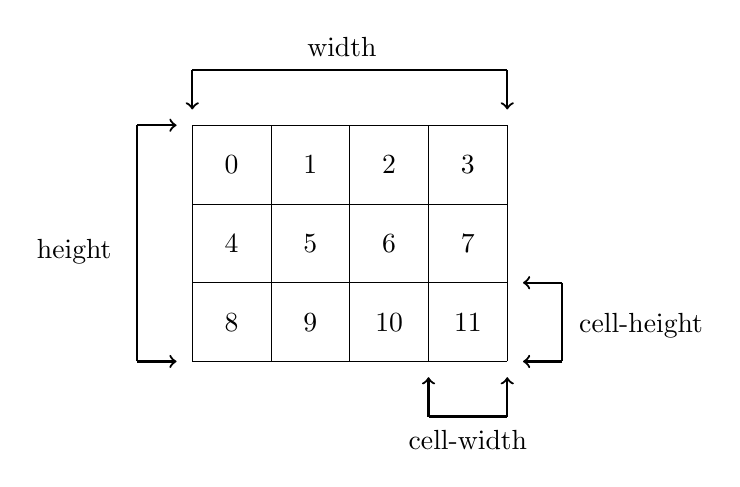
\begin{tikzpicture}
        \draw[step=1cm,black,very thin] (0,0) grid (4,3);
        \draw[thick,->] (-0.7,3) -- (-0.2,3);
        \draw[thick] (-0.7,3) -- (-0.7,0);
        \draw[thick,->] (-0.7,0) -- (-0.2,0);
        \draw (-1.5,1.4) node{height};

        \draw[thick,->] (0,3.7) -- (0,3.2);
        \draw[thick] (0,3.7) -- (4,3.7);
        \draw[thick,->] (4,3.7) -- (4,3.2);
        \draw (1.9,4) node{width};

        \draw[thick,->] (4.7,1) -- (4.2,1);
        \draw[thick] (4.7,1) -- (4.7,0);
        \draw[thick,->] (4.7,0) -- (4.2,0);
        \draw (5.7,0.45) node{cell-height};

        \draw[thick,->] (3,-0.7) -- (3,-0.2);
        \draw[thick] (3,-0.7) -- (4,-0.7);
        \draw[thick,->] (4,-0.7) -- (4,-0.2);
        \draw (3.5, -1) node{cell-width};

        \draw (0.5, 2.5) node{0};
        \draw (1.5, 2.5) node{1};
        \draw (2.5, 2.5) node{2};
        \draw (3.5, 2.5) node{3};

        \draw (0.5, 1.5) node{4};
        \draw (1.5, 1.5) node{5};
        \draw (2.5, 1.5) node{6};
        \draw (3.5, 1.5) node{7};

        \draw (0.5, 0.5) node{8};
        \draw (1.5, 0.5) node{9};
        \draw (2.5, 0.5) node{10};
        \draw (3.5, 0.5) node{11};
    \end{tikzpicture}
\end{center}

\subsubsection{DisplayChangeReceived - TCP}

The DisplayChangeReceived message is sent in reply after receiving a DisplayChange message. It
indicates to the Host they may start sending FrameData referencing the new DisplayInformation in
the most recent DisplayChange.

\begin{center}
    Client \textrightarrow\ Host\\
    \begin{tabular}{|c|c|c|}
        \hline
        \textbf{Bytes} & \textbf{Name} & \textbf{Value} \\
        \hline
        1              & type          & 2              \\
        \hline
    \end{tabular}
\end{center}

\subsubsection{MouseLocation - TCP/UDP}

The \emph{MouseLocation} message send information about where the mouse is currently on the screen.
The Host sends this information periodically throughout the session.
The Host SHOULD send a \emph{MouseLocation} update when mouse input is received from the Host's system or in
reply when it receives a \emph{MouseInput}.

\begin{center}
    Host \textrightarrow\ Client\\
    \begin{tabular}{|c|c|c|c|}
        \hline
        \textbf{Bytes} & \textbf{Name} & \textbf{Value} & \textbf{Description}      \\
        \hline
        3              & type          & 3              &                           \\
        \hline
        1              & display-id    & 0-255          &                           \\
        \hline
        2              & x-location    &                & x coordinate of the mouse \\
        \hline
        2              & y-location    &                & y coordinate of the mouse \\
        \hline
    \end{tabular}
\end{center}

\subsection{Input}

Input messages (including \emph{MouseLocation}) may be sent over TCP or UDP. TCP is preferred in most situations.
However, in situations where speed is prioritized over the guarantees TCP provides (such as gaming), UDP can be
used.

\subsubsection{MouseInput - TCP/UDP}

\begin{center}
    Client \textrightarrow\ Host\\
    \begin{tabular}{|c|c|c|c|}
        \hline
        \textbf{Bytes} & \textbf{Name} & \textbf{Value} & \textbf{Description}      \\
        \hline
        1              & type          & 4              &                           \\
        \hline
        1              & display-id    & 0-255          &                           \\
        \hline
        2              & x-position    &                & x coordinate of the mouse \\
        \hline
        2              & y-position    &                & y coordinate of the mouse \\
        \hline
        1              & button-mask   &                & described below           \\
        \hline
    \end{tabular}
\end{center}

%  https://github.com/rfbproto/rfbproto/blob/master/rfbproto.rst#pointerevent %
Indicates either pointer movement or a pointer button press or release. The pointer is now at (x-position,
y-position), and the current state of buttons 1 to 8 are represented by bits 0 to 7 of button-mask respectively,
0 meaning up, 1 meaning down (pressed).\\

On a conventional mouse, buttons 1, 2 and 3 correspond to the left, middle and right buttons on the mouse. On a
wheel mouse, each step of the wheel is represented by a press and release of a certain button. Button 4 means up,
button 5 means down, button 6 means left and button 7 means right.

\subsubsection{KeyInput - TCP/UDP}

The \emph{KeyInput} event sends key presses or releases.

\begin{center}
    Client \textrightarrow\ Host\\
    \begin{tabular}{|c|c|c|c|}
        \hline
        \textbf{Bytes} & \textbf{Name} & \textbf{Value} & \textbf{Description}                                 \\
        \hline
        1              & type          & 5              &                                                      \\
        \hline
        1              & down-flag     & 0 or 1         & indicates whether the key is now pressed or released \\
        \hline
        4              & key           &                & "keysym"                                             \\
        \hline
    \end{tabular}
\end{center}

Details can be found at the \href{https://github.com/rfbproto/rfbproto/blob/master/rfbproto.rst#keyevent}{RFB Spec}

\subsection{Clipboard}

\subsubsection{ClipboardRequest - TCP}

Used to check if a clipboard type exists on the Host.

\begin{center}
    Client \textrightarrow\ Host\\
    \begin{tabular}{|c|c|c|}
        \hline
        \textbf{Bytes}   & \textbf{Name}    & \textbf{Value} \\
        \hline
        1                & type             & 6              \\
        \hline
        1                & clipboard-type   &                \\
        \hline
        \multicolumn{3}{|c|}{\textbf{Below only if clipboard-type's first bit is 1} } \\
        \hline
        1                & type-name-length &                \\
        \hline
        type-name-length & type-name        &                \\
        \hline
    \end{tabular}
\end{center}

clipboard-type's first bit indicates whether this request is for a default type (\texttt{0}) or a custom type
(\texttt{1}). clipboard-type's second bit indicates whether this request is a exists request (\texttt{0}) or a
content request(\texttt{1}). An exists request is for checking whether the type exists but does not return content. A
content request returns content if it exists. The remaining bits indicate the default type if the request is for a
default type. Otherwise they are ignored.\\

clipboard-type's remaining bits referring to the following default types:

\begin{center}
    \begin{tabular}{|c|c|}
        \hline
        \textbf{Value} & \textbf{Description} \\
        \hline
        0              & text                 \\
        \hline
        1              & rtf                  \\
        \hline
        2              & html                 \\
        \hline
        3              & file-pointer         \\
        \hline
    \end{tabular}
\end{center}

\subsubsection{ClipboardNotification- TCP}

Notifies a Peer of a clipboard update. The receiving Peer should update their clipboard.

\begin{center}
    Host $\leftrightarrow$ Client\\
    \begin{tabular}{|c|c|c|}
        \hline
        \textbf{Bytes}        & \textbf{Name}    & \textbf{Value}   \\
        \hline
        1                     & type             & 7                \\
        \hline
        1                     & clipboard-type   &                  \\
        \hline
        \multicolumn{3}{|c|}{\textbf{Below only if clipboard-type's first bit is 1} } \\
        \hline
        1                     & type-name-length &                  \\
        \hline
        type-name-length      & type-name        &                  \\
        \hline
        \multicolumn{3}{|c|}{\textbf{Below only if clipboard-type's second bit is 1} } \\
        3                     & content-length   &                  \\
        \hline
        \emph{content-length} & data             & zlib'ed raw data \\
        \hline
    \end{tabular}
\end{center}


clipboard-type, type-name-length, and type-name MUST match a request if the notification is in response. If
clipboard-readable is 0 and a Host receives a ClipboardRequest, it MUST be ignored. If no Display is Controllable or
clipboard-readable is 0 and a Host receives a ClipboardNotification, it MUST be ignored.\\

content-length -  the length of the content  (maximum $2^{24}$ bytes or ~16MB )\\

\subsection{FrameData - UDP}
The \emph{FrameData} message contains an update of a particular cell on a particular \emph{Display}.

\begin{center}
    Host \textrightarrow Client\\
    \begin{tabular}{|c|c|c|}
        \hline
        \textbf{Bytes} & \textbf{Name} & \textbf{Value} \\
        \hline
        1              & type          & 8             \\
        \hline
        4              & frame-number  &                \\
        \hline
        1              & display-id    & 0-255          \\
        \hline
        2              & cell-number   &                \\
        \hline
        2              & size          &                \\
        \hline
        \emph{size}    & data          &                \\
        \hline
    \end{tabular}
\end{center}

\emph{frame-number} is a 32 bit counter, initialized with 0 at the beginning of the protocol, and incremented once
from \emph{FrameData} message sent.

\emph{data} contains raw RGB pixel data of the updated cell.

\subsection{Congestion}

When sending messages over a network the network may become congested to avoid congesting the network further RVD
implements a congestion detection and congestion control mechanism. RVD uses Additive increase/multiplicative
decrease or AIMD to control the \emph{OutputMaximum} which is the maximum messages allowed per
\emph{CongestionWindow}.

\end{document}
